% =============================================================================
%  Section: Radiative Corrections
%  H1 Charged-Hadron SIDIS High-Q^2 Analysis Note
% =============================================================================
\section{Radiative Corrections}
\label{sec:radiative_corrections}

In addition to the hard scattering process itself, the incoming or the
outgoing lepton can emit real photons (QED radiation from the lepton
line).  Such photon emission changes the energy and the direction of the
scattered lepton and thereby shifts the event kinematics reconstructed
from it, so the measured cross section differs from the Born-level cross
section, i.e. the cross section of the hard scattering process with no
photon emitted from the lepton line.  A per-bin radiative correction
factor, $C_{\mathrm{rad}}$, converts the measured cross section to the
Born level.

\subsection{Definition and Derivation}
\label{sec:radiative_corrections:definition}

The correction is defined, separately in each published bin of the
analysis, as the ratio
\begin{equation}
  C_{\mathrm{rad}}(\mathrm{bin}) =
  \frac{\sigma_{\mathrm{nonrad}}(\mathrm{bin})}
       {\sigma_{\mathrm{rad}}(\mathrm{bin})},
\end{equation}
where $\sigma_{\mathrm{rad}}$ and $\sigma_{\mathrm{nonrad}}$ are the
generator-level cross sections that the same event generator predicts in
the same bin when photon emission from the lepton line is switched on and
off, respectively.  Each of the two cross sections is computed as the
weighted generator-level event yield in the bin, normalised by the
integrated luminosity of the corresponding simulated sample; only these
two simulated luminosities enter the ratio, and the data luminosity does
not enter at all.  The two samples are processed with an identical event
selection, identical binning, the same charged-hadron definition, and the
same event weighting, so that the ratio isolates the effect of the photon
radiation.  No detector simulation enters the derivation: the correction
is a purely generator-level quantity.

The correction is derived independently with two event generators, DJANGOH
\cite{Charchula:1994kf} and RAPGAP \cite{Jung:1993gf}, both of which are
interfaced to the same QED-radiation program, HERACLES
\cite{Kwiatkowski:1990es}, so that each generator can produce a matched
pair of samples with and without photon emission from the lepton line.
The DJANGOH correction is the one applied to the data.  The RAPGAP
correction is retained as an independent comparison and determines the
generator-related uncertainty of the correction
(Sec.~\ref{sec:radiative_corrections:uncertainties}).

Both samples of a pair are subject to the generator-level counterpart of
the analysis selection, so that the correction corresponds to the same
phase space and the same hadron population as the measurement.  The
selection comprises the DIS kinematic requirements of the measurement,
$150<\Qsq<20\,000~\GeVsq$ and $0.1<y<0.7$
(Sec.~\ref{sec:selection:final-events}); a minimum requirement on the
total hadronic final-state energy--momentum balance, $E-p_z>45~\GeV$; and
the current-hemisphere requirement that the hadron lie in the
current-fragmentation hemisphere of the $\gamma^{*}p$ center-of-mass
frame---the hemisphere into which the struck quark fragments, opposite
the proton-remnant direction---which corresponds to $x_F<0$ in the H1
sign convention used throughout this analysis
(Sec.~\ref{sec:selection:final-tracks}).  Every element of the selection,
in particular the current-hemisphere requirement, is imposed identically
on the radiative and the non-radiative sample.  The charged hadrons are
pions, kaons, and (anti)protons, the same truth-level hadron definition
as in the measurement (Sec.~\ref{sec:species_definition}), and the two
beam charges are combined in both samples, matching the combined
$e^{+}p$ and $e^{-}p$ data set of the measurement.

The current correction tables supersede all earlier versions.  They are the
releasebin tables, in which events are assigned to $(Q2esGen,x_{\mathrm{es,gen}})$
bins with the same definition of $x$ as the release binning.  The applied
DJANGOH14 table is
\path{/data/dust/group/h1/klesthen/BaryonAsym/sidis_highQ2/data/radiative/djangoh14_crad_releasebin_2026-10-09/crad_v3_xfgen_lt0_empz_gt45_nominal_490rows.csv};
the formal RAPGAP31 alternative is
\path{/data/dust/group/h1/klesthen/BaryonAsym/sidis_highQ2/data/radiative/rapgap_crad_releasebin_emfix_2026-10-09/crad_v3_xfgen_lt0_empz_gt45_nominal_490rows.csv}.
The current-hemisphere requirement and the EMPZ$>$45 convention are unchanged.

\subsection{Correction Factors}
\label{sec:radiative_corrections:values}

Integrated over all 490 published bins, the applied DJANGOH correction is
$1.142$ for $\hplus$ and $1.141$ for
$\hminus$.  The corresponding RAPGAP factors are $1.134$
for $\hplus$ and $1.134$ for $\hminus$.  For both
generators, every one of the 490 bins (245 per charge) has a finite
entry.  Integrated over all bins, the DJANGOH correction exceeds the
RAPGAP correction by $0.6419\%$ for $\hplus$ and $0.6499\%$ for
$\hminus$.

The precision of the correction itself is limited by the number of
simulated events.  The per-bin relative statistical uncertainty of the
applied correction has a median of $0.4272\%$ for $\hplus$ and
$0.4429\%$ for $\hminus$.

Table~\ref{tab:crad:integrated-variants} compares the integrated factors of
the applied mixed-beam correction with those of the two derived Born-target
variants, together with their integrated statistical uncertainties and,
where a RAPGAP31 counterpart exists, the integrated generator difference.
The two target variants are provisional diagnostics and are not applied to
any result in this note.

\begin{table}[h]
\centering
\small
\begin{tabular}{p{4.6cm}p{5.2cm}p{5.2cm}}
\toprule
Variant & $\hplus$ & $\hminus$ \\
\midrule
Mixed-beam (applied primary, DJANGOH14 releasebin)$^{a}$ &
  $1.142 \pm 0.000123$ (stat) $\pm 0.00728$ (gen) &
  $1.141 \pm 0.000124$ (stat) $\pm 0.00736$ (gen) \\
$e^{-}p$ WithZ (per-beam target, DJANGOH14)$^{b}$ &
  $1.148 \pm 0.000151$ (stat) $\pm 0.0106$ (gen) &
  $1.147 \pm 0.000151$ (stat) $\pm 0.0101$ (gen) \\
NoZ photon-Born $C_{\gamma\mathrm{Born}}$ (DJANGOH14)$^{c}$ &
  $1.041 \pm 0.000143$ (stat) &
  $1.040 \pm 0.000144$ (stat) \\
\bottomrule
\end{tabular}

{\footnotesize
$^{a}$The applied primary: the per-bin DJANGOH14 releasebin tables applied
to the Born release (Sec.~\ref{sec:radiative_corrections:application}); the
Born level is the luminosity-weighted mixture of the $e^{+}p$ and $e^{-}p$
Born cross sections.

\smallskip
$^{b}$A pure $e^{-}p$ full-electroweak (WithZ) Born target, derived with the
per-bin factor $F_{\mathrm{exact}}$ and the current beam split
$f_{e^{+}p} = 0.5440407473$, $f_{e^{-}p} = 0.4559592527$; provisional
diagnostic, not applied (derivation record
\path{/data/dust/group/h1/klesthen/BaryonAsym/sidis_highQ2/docs/radiative/EMINUS_WITHZ_CRAD_DERIVATION_2026-10-19.md}).

\smallskip
$^{c}$The photon-only Born target, with the $Z$-boson couplings zeroed
(Sec.~\ref{sec:radiative_corrections:photon-born-variant}); DJANGOH-only,
because no corresponding photon-only RAPGAP sample exists, so that no
generator uncertainty is derivable; provisional diagnostic, not applied.

\smallskip
$^{d}$The integrated statistical uncertainties are leg-level bookkeeping
numbers that assume per-leg weighted statistics independent across bins;
they are not an event-level covariance propagation (method record
\path{/data/dust/group/h1/klesthen/BaryonAsym/sidis_highQ2/docs/radiative/integrated_stat_unc_method_2026-10-19.md};
full-precision source
\path{/data/dust/group/h1/klesthen/BaryonAsym/sidis_highQ2/data/radiative/eminus_withz_crad_releasebin_2026-10-19/integrated_stat_unc_for_note_2026-10-19.json}).
\par}

\caption{Comparison of the integrated $C_{\mathrm{rad}}$ values of the
applied correction and of the two derived Born-target variants, in the
ratio-of-integrals convention over the 245 published bins of each charge.
The central value is the DJANGOH14 factor; the first uncertainty is the
integrated statistical uncertainty propagated from the DJANGOH14
legs,$^{d}$ and the second is the full integrated absolute
DJANGOH14--RAPGAP31 difference.}
\label{tab:crad:integrated-variants}
\end{table}

\subsection{Application to the Measurement}
\label{sec:radiative_corrections:application}

For the current release, in which the background-subtracted data vector is
unfolded with the response's own generator-level prior, the correction is
applied bin by bin
after the unfolding of the detector response and converts the unfolded cross
section to the Born level:
\begin{equation}
  \sigma_{\mathrm{Born}}(\mathrm{bin}) =
  C_{\mathrm{rad}}(\mathrm{bin}) \times
  \sigma_{\mathrm{unfolded}}(\mathrm{bin}).
\end{equation}
All cross sections quoted in this note are Born-level cross sections
obtained in this way, unless explicitly stated otherwise.  The release to
which the correction is applied is described in
Sec.~\ref{sec:results:z005-release}.  The correction has been applied to
all released cross sections since its derivation was completed in
October 2026; cross sections produced before the correction was applied
are superseded.

\subsection{Uncertainties}
\label{sec:radiative_corrections:uncertainties}

Two components of the systematic uncertainty are associated with the
radiative correction and enter the total systematic budget of
Sec.~\ref{sec:systematics}.  The first component describes the difference
between the two generators: the bin-by-bin difference between the DJANGOH
and RAPGAP corrections is carried as a systematic uncertainty, with a
median of $0.5844\%$ ($\hplus$) and $0.5804\%$ ($\hminus$) and a maximum
of $5.762\%$ and $5.663\%$, respectively.  The second component is the
statistical uncertainty of the correction itself, carried as a separate
systematic uncertainty bin by bin, with the per-bin medians quoted
above.

\subsection{Status and Caveats}
\label{sec:radiative_corrections:caveats}

The correction is applied to all released cross sections, but it does not
yet have publication-grade status.  The following caveats apply:
\begin{itemize}
  \item the correction tables retain provisional status pending a final
        publication review;
  \item the exposure of the simulated samples is reconciled file by file with
        the stored event lists, while the cross-check against the original
        generator production logs remains open;
  \item the correction is derived from, and valid for, the combined
        $e^{+}p$ and $e^{-}p$ data set only; it is neither a per-beam-charge
        correction nor an $e^{-}$ Born target correction;
  \item the sensitivity of the correction to the exact hadronic
        energy--momentum balance requirement was studied, and the chosen
        threshold of $E-p_z>45~\GeV$ was retained;
  \item differences between variants of the correction that differ in the
        exact definition of the current-hemisphere requirement concentrate
        in the lowest $z$ bin ($z<0.05$): there the per-bin sensitivity
        reaches $9.9\%$ ($\hplus$) and $8.0\%$ ($\hminus$) for DJANGOH
        and $6.5\%$ and $5.2\%$ for RAPGAP, while above $z=0.05$ the
        median effect is zero.
\end{itemize}

% TODO: reinstate generator-comparison figures once regenerated from the current correction tables
% \begin{figure}[p]
%   \centering
%   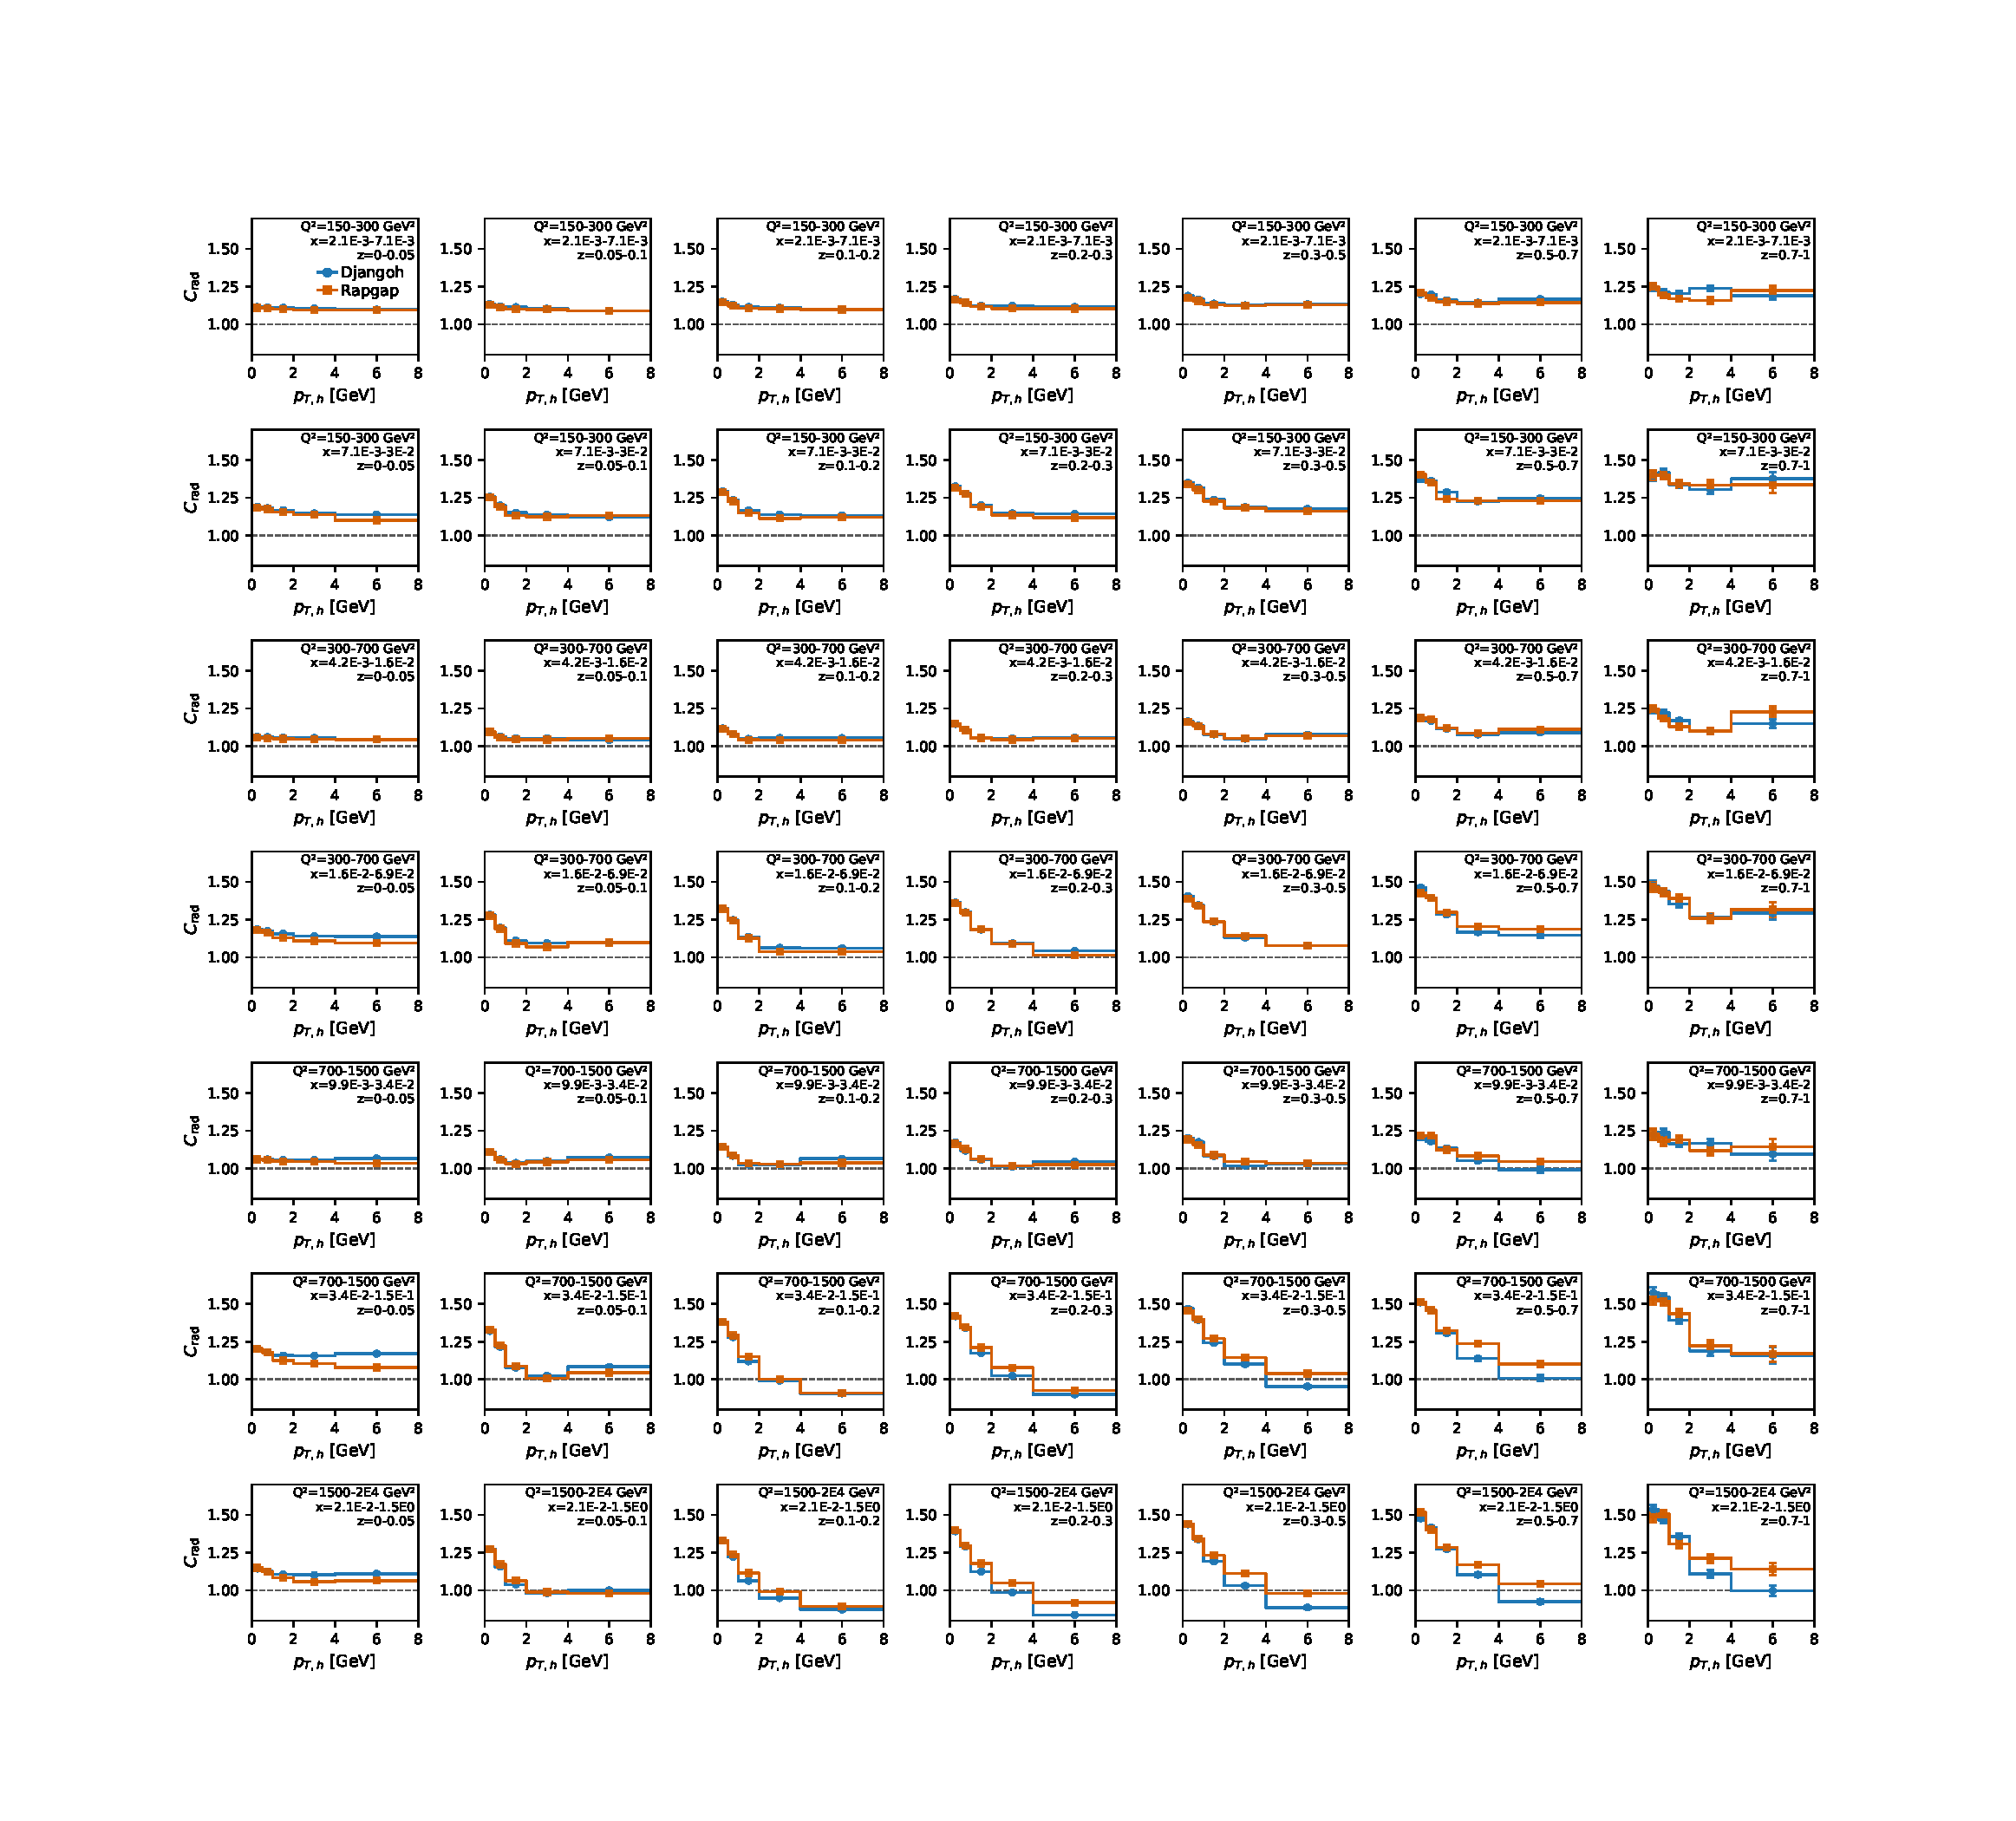
\includegraphics[width=1.05\textwidth,height=0.82\textheight,keepaspectratio]{figures/crad_djangoh14_vs_rapgap31_fLumi_v3_7col_hplus_zoom.pdf}
%   \caption{Comparison of $C_{\mathrm{rad}}=\sigma_{\mathrm{nonrad}}/\sigma_{\mathrm{rad}}$ for DJANGOH14 and RAPGAP31 for $\hplus$.}
%   \label{fig:crad:djangoh-rapgap-flumi-v3-hplus}
% \end{figure}
%
% \begin{figure}[p]
%   \centering
%   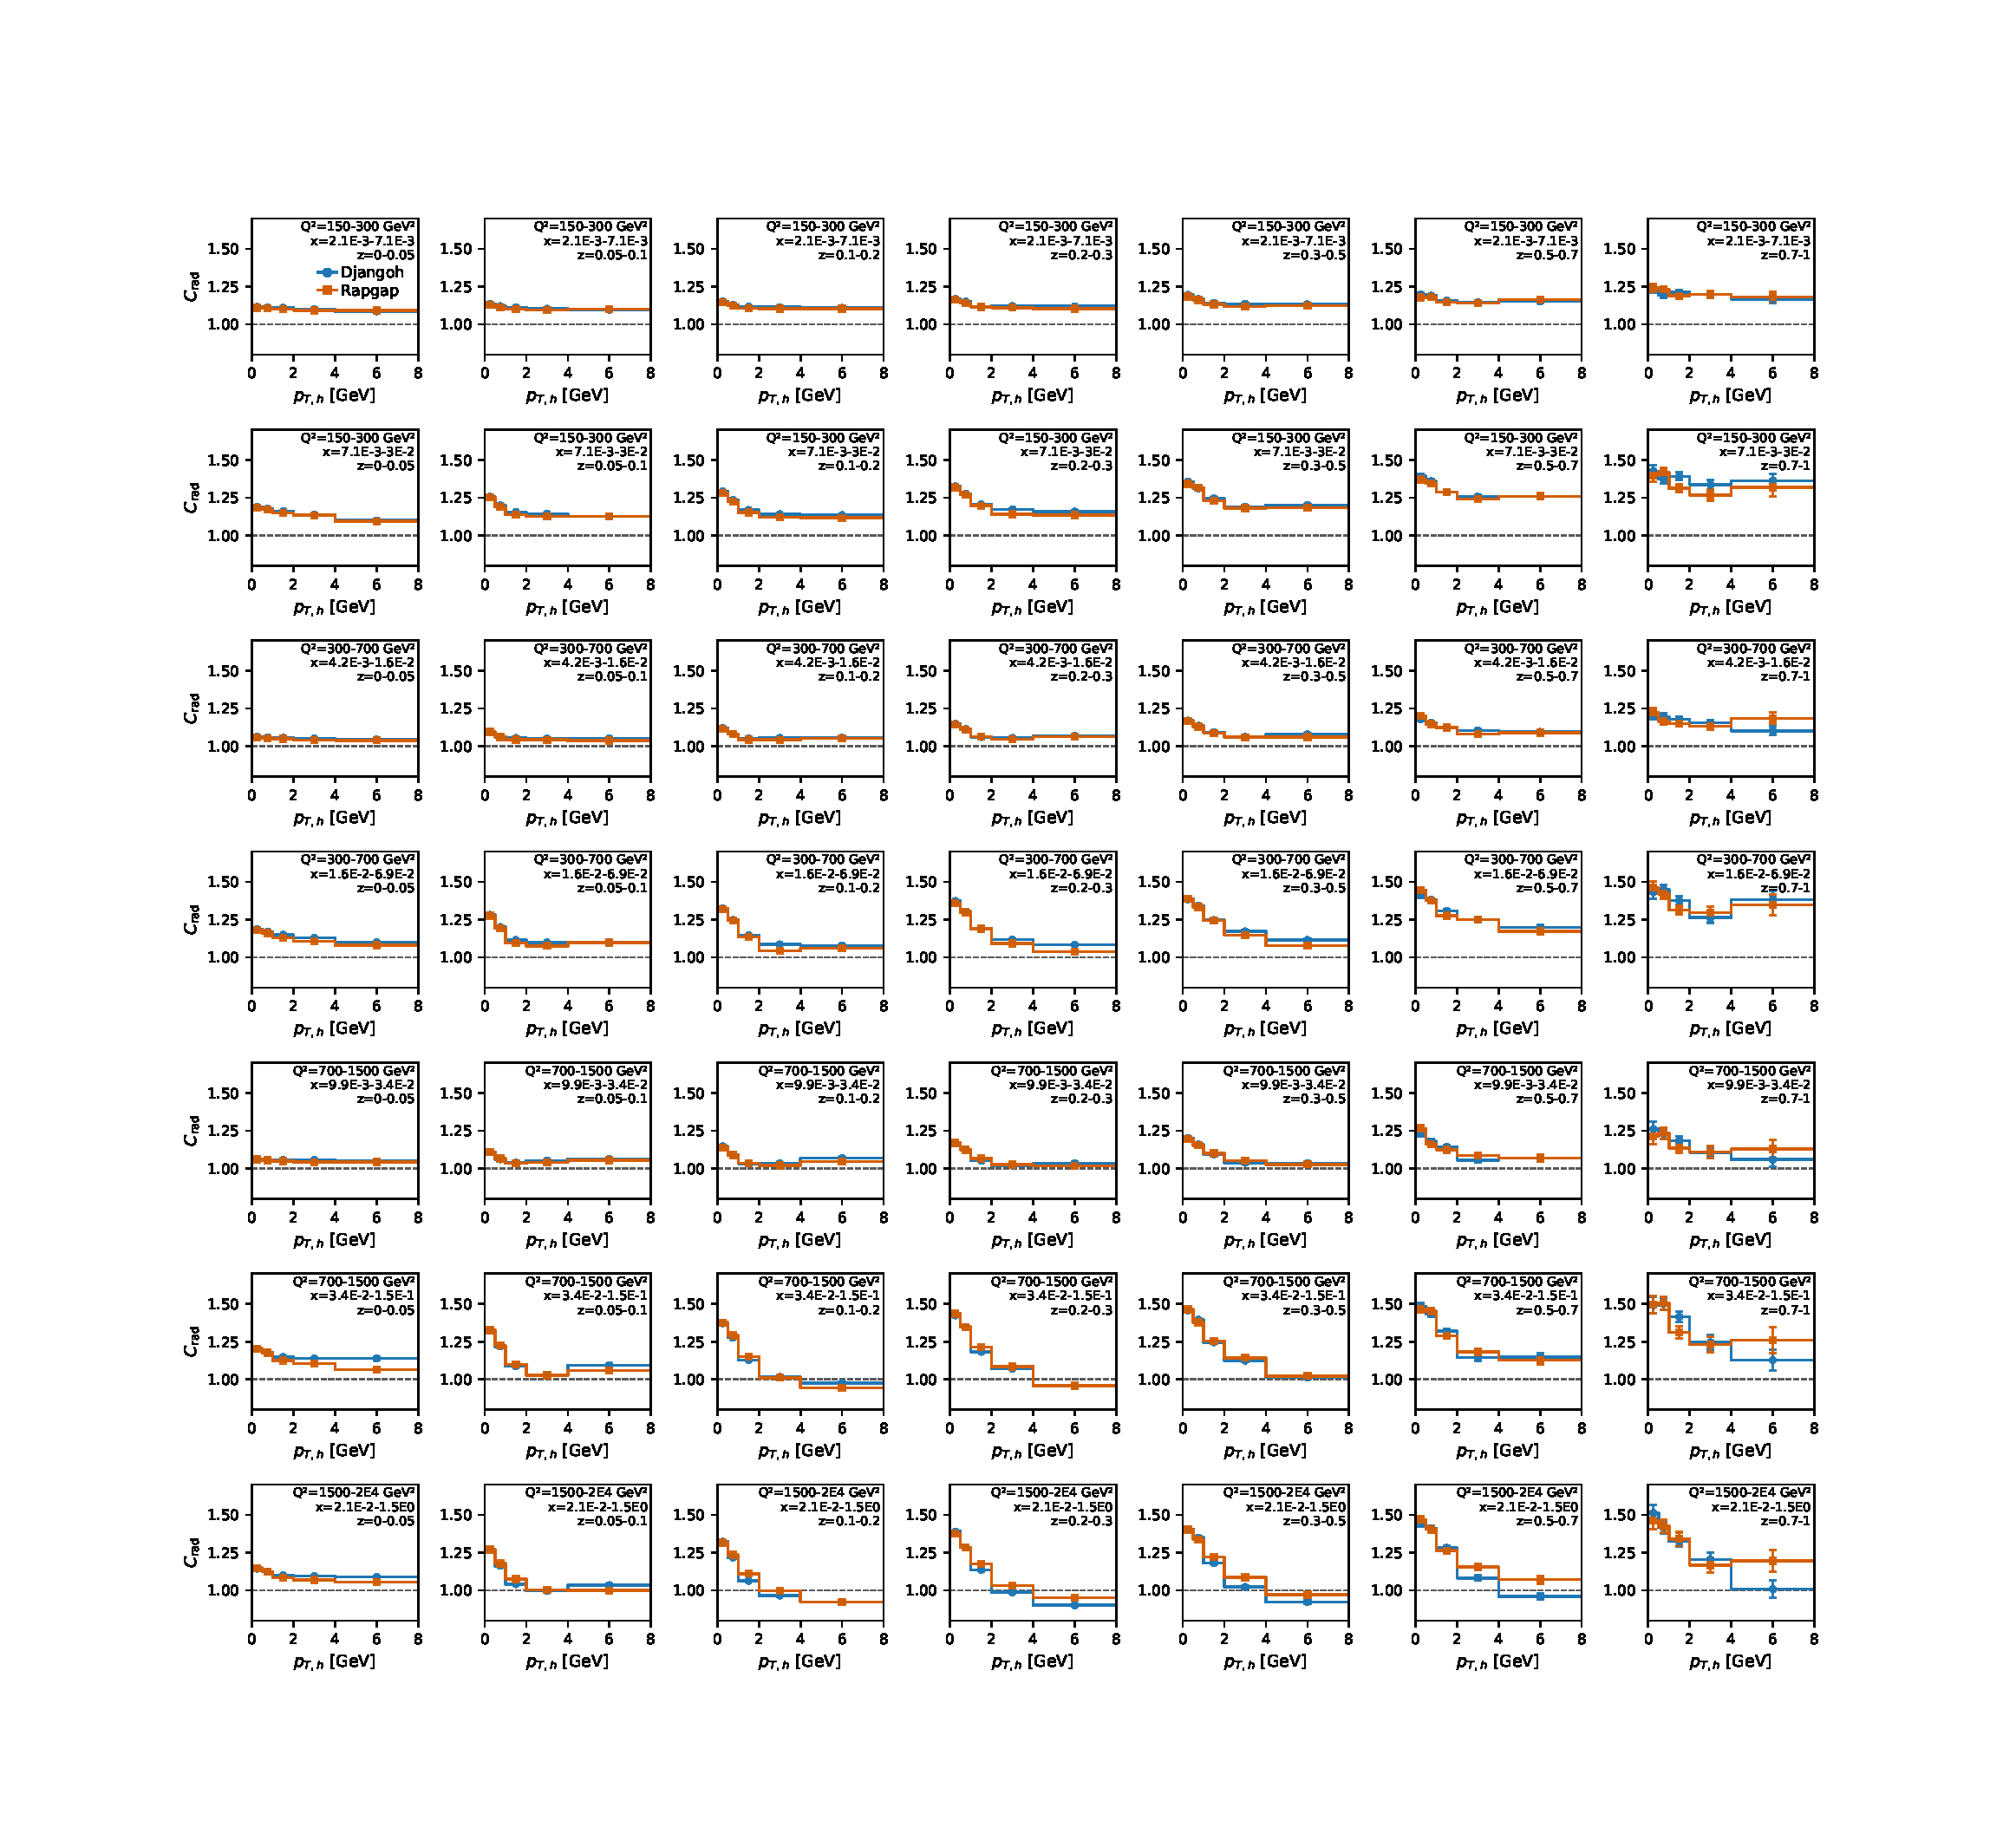
\includegraphics[width=1.05\textwidth,height=0.82\textheight,keepaspectratio]{figures/crad_djangoh14_vs_rapgap31_fLumi_v3_7col_hminus_zoom.pdf}
%   \caption{Comparison of $C_{\mathrm{rad}}=\sigma_{\mathrm{nonrad}}/\sigma_{\mathrm{rad}}$ for DJANGOH14 and RAPGAP31 for $\hminus$.}
%   \label{fig:crad:djangoh-rapgap-flumi-v3-hminus}
% \end{figure}

\subsection{Photon-Only Born Variant $C_{\gamma\mathrm{Born}}$}
\label{sec:radiative_corrections:photon-born-variant}

The Born level used for all results in this note is the Born level of the
full neutral-current process, with both photon and $Z$-boson exchange.
As a diagnostic variant, a second per-bin correction,
$C_{\gamma\mathrm{Born}}$, was derived with the same method, selection,
and binning, mapping the measured cross section instead to a Born level
of pure photon exchange, in which the $Z$-boson contribution is absent.
Its integrated factors are $1.041$ for $\hplus$ and
$1.040$ for $\hminus$; they are smaller than the
$C_{\mathrm{rad}}$ factors because the target level itself is lower, not
because of a different treatment of the photon radiation.  This variant
is a provisional diagnostic product: it is not applied to any result in
this note, and it is derived with DJANGOH only, because no corresponding
photon-only RAPGAP sample exists, so the generator comparison that backs
the main correction is not available for the variant.  The two
corrections map the same measurement to different Born conventions and
must not be composed, averaged, or interchanged; any quoted cross section
must state which of the two Born conventions it uses.
